% da valutare se questa cosa è solo per il tecnico

\subsubsection{UC9 - Visualizzazione lista dizionari dati caricati nel sistema}\label{UC9}

\begin{figure}[H]
  \centering
  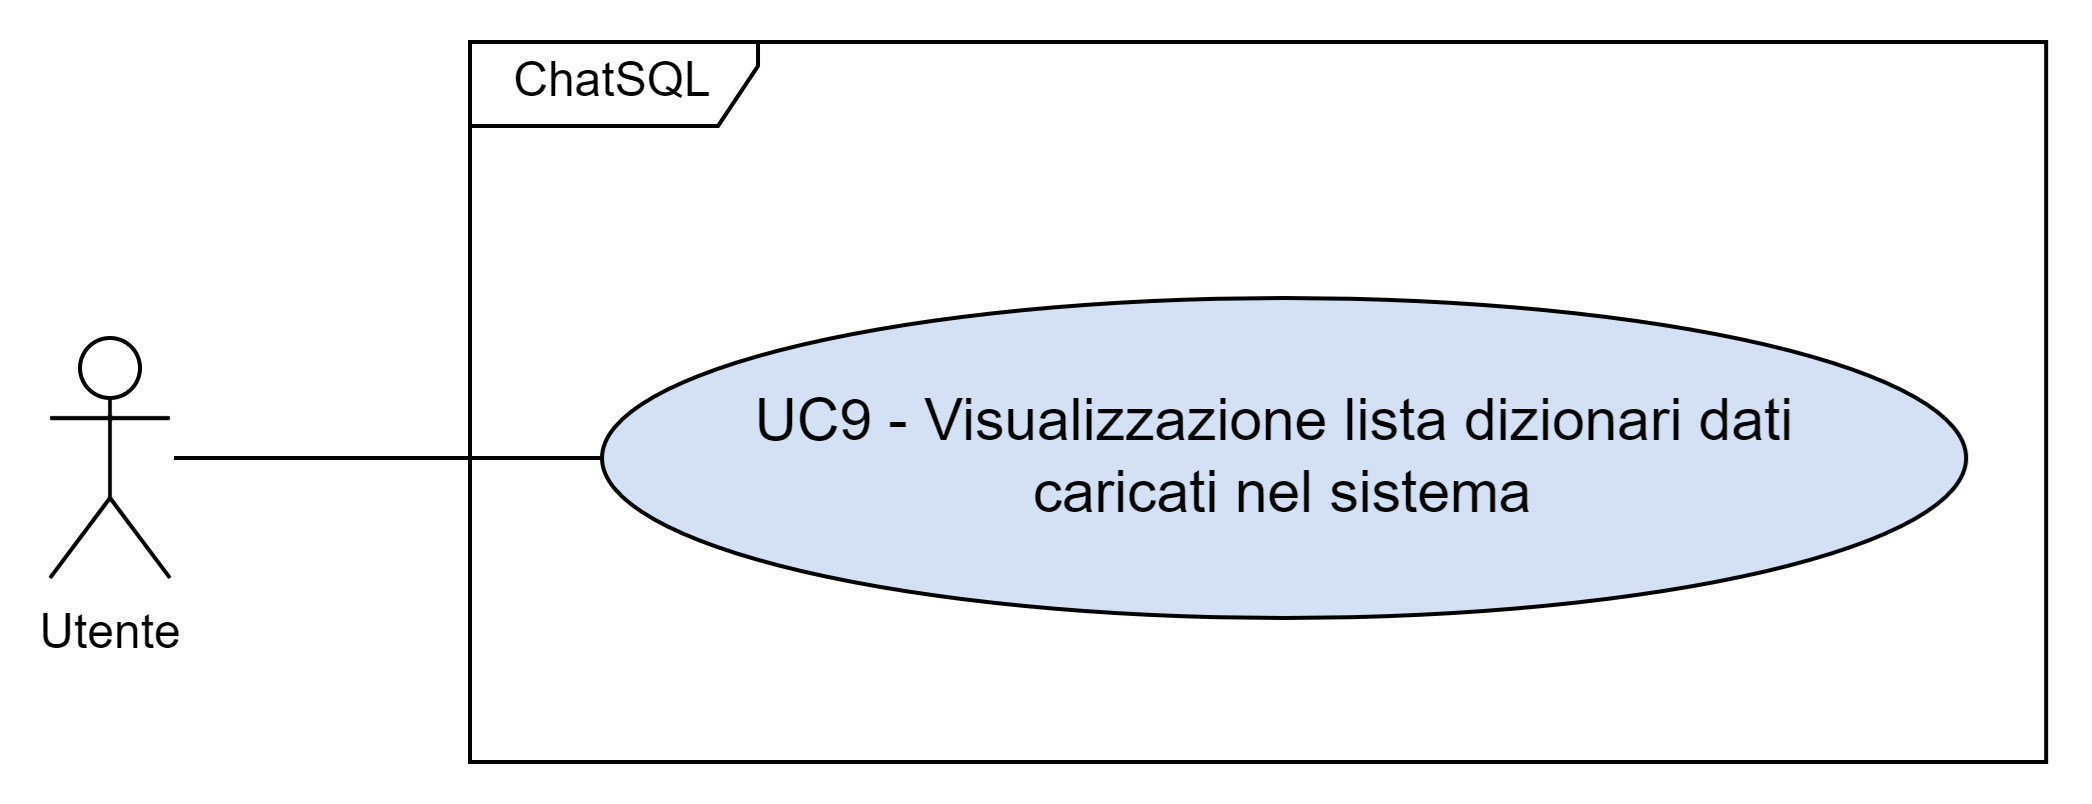
\includegraphics[width=0.90\textwidth]{assets/uc9.png}
  \caption{UC9}
\end{figure}

\paragraph*{Descrizione}
L'Utente visualizza la lista dei \glossario{dizionari dati} che sono stati caricati nel sistema.

\paragraph*{Attori principali}
Utente

\paragraph*{Precondizioni}
\begin{itemize}
  \item Il sistema è attivo e funzionante;
  \item È stato caricato almeno un \glossario{dizionario dati}.  
\end{itemize}

\paragraph*{Postcondizioni}
\begin{itemize}
\item Viene visualizzata la lista dei \glossario{dizionari dati} presenti nel sistema.
\end{itemize}

\paragraph*{Trigger}
L'Utente desidera visualizzare i \glossario{dizionari dati} disponibili.

\paragraph*{Scenario principale}
\begin{enumerate}
  \item L'Utente visualizza la lista dei \glossario{dizionari dati}.
\end{enumerate}

\paragraph*{Sottocasi d'uso:}
\begin{enumerate}
  \item UC9.1: Visualizzazione singolo dizionario dati.
\end{enumerate}

\begin{figure}[H]
  \centering
  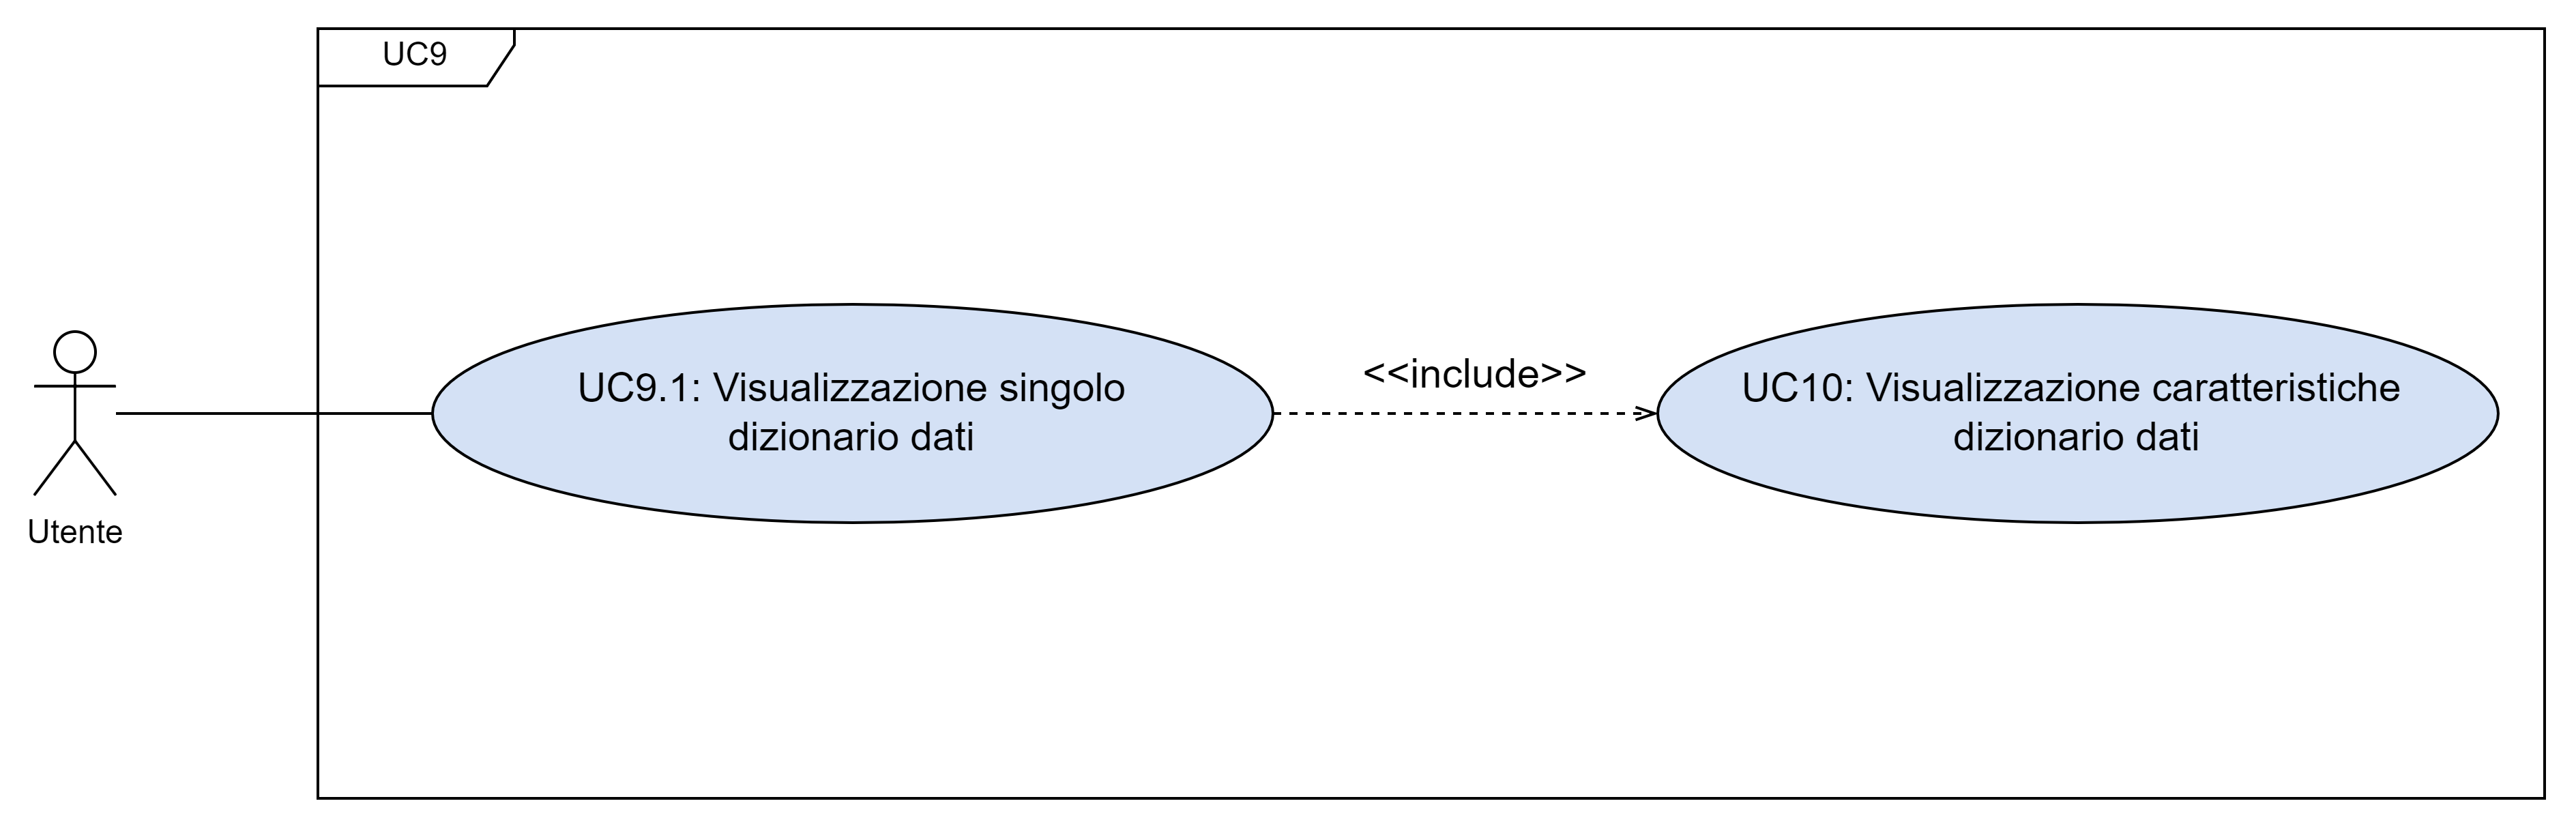
\includegraphics[width=0.90\textwidth]{assets/uc9_1.png}
  \caption{UC9 - Sottocasi d'uso}
\end{figure}

%%%%%%%%%%%%%%%%%%%%%%%%%%%%%%%%%%%%%%%%%%%%%%%%%%%%%%%%%%%%%%%%%%%%%%%%%%%%%%

\subsubsection{UC9.1 - Visualizzazione singolo dizionario dati}\label{UC9point1}
\paragraph*{Descrizione}
L'Utente visualizza un dizionario all'interno della lista dei \glossario{dizionari dati} caricati nel sistema.

\paragraph*{Attori principali}
Utente

\paragraph*{Precondizioni}
\begin{itemize}
  \item Il sistema è attivo e funzionante;
  \item È stato caricato almeno un \glossario{dizionario dati};
  \item È visibile la lista dei \glossario{dizionari dati} (\hyperref[UC9]{UC9}).
\end{itemize}

\paragraph*{Postcondizioni}
\begin{itemize}
  \item Viene visualizzato correttamente il \glossario{dizionario dati}.
\end{itemize}

\paragraph*{Trigger}
L'Utente desidera visualizzare un dizionario all'interno della lista.

\paragraph*{Scenario principale}
\begin{enumerate}
  \item L'Utente visualizza un singolo \glossario{dizionario dati}.
\end{enumerate}

\paragraph*{Inclusioni}
\begin{itemize}
  \item Visualizzazione caratteristiche \glossario{dizionario dati} (\hyperref[UC10]{UC10});
\end{itemize}